\documentclass[]{elsarticle} %review=doublespace preprint=single 5p=2 column
%%% Begin My package additions %%%%%%%%%%%%%%%%%%%
\usepackage[hyphens]{url}

  \journal{An awesome journal} % Sets Journal name


\usepackage{lineno} % add
\providecommand{\tightlist}{%
  \setlength{\itemsep}{0pt}\setlength{\parskip}{0pt}}

\usepackage{graphicx}
\usepackage{booktabs} % book-quality tables
%%%%%%%%%%%%%%%% end my additions to header

\usepackage[T1]{fontenc}
\usepackage{lmodern}
\usepackage{amssymb,amsmath}
\usepackage{ifxetex,ifluatex}
\usepackage{fixltx2e} % provides \textsubscript
% use upquote if available, for straight quotes in verbatim environments
\IfFileExists{upquote.sty}{\usepackage{upquote}}{}
\ifnum 0\ifxetex 1\fi\ifluatex 1\fi=0 % if pdftex
  \usepackage[utf8]{inputenc}
\else % if luatex or xelatex
  \usepackage{fontspec}
  \ifxetex
    \usepackage{xltxtra,xunicode}
  \fi
  \defaultfontfeatures{Mapping=tex-text,Scale=MatchLowercase}
  \newcommand{\euro}{€}
\fi
% use microtype if available
\IfFileExists{microtype.sty}{\usepackage{microtype}}{}
\bibliographystyle{elsarticle-harv}
\usepackage{color}
\usepackage{fancyvrb}
\newcommand{\VerbBar}{|}
\newcommand{\VERB}{\Verb[commandchars=\\\{\}]}
\DefineVerbatimEnvironment{Highlighting}{Verbatim}{commandchars=\\\{\}}
% Add ',fontsize=\small' for more characters per line
\usepackage{framed}
\definecolor{shadecolor}{RGB}{248,248,248}
\newenvironment{Shaded}{\begin{snugshade}}{\end{snugshade}}
\newcommand{\AlertTok}[1]{\textcolor[rgb]{0.94,0.16,0.16}{#1}}
\newcommand{\AnnotationTok}[1]{\textcolor[rgb]{0.56,0.35,0.01}{\textbf{\textit{#1}}}}
\newcommand{\AttributeTok}[1]{\textcolor[rgb]{0.77,0.63,0.00}{#1}}
\newcommand{\BaseNTok}[1]{\textcolor[rgb]{0.00,0.00,0.81}{#1}}
\newcommand{\BuiltInTok}[1]{#1}
\newcommand{\CharTok}[1]{\textcolor[rgb]{0.31,0.60,0.02}{#1}}
\newcommand{\CommentTok}[1]{\textcolor[rgb]{0.56,0.35,0.01}{\textit{#1}}}
\newcommand{\CommentVarTok}[1]{\textcolor[rgb]{0.56,0.35,0.01}{\textbf{\textit{#1}}}}
\newcommand{\ConstantTok}[1]{\textcolor[rgb]{0.00,0.00,0.00}{#1}}
\newcommand{\ControlFlowTok}[1]{\textcolor[rgb]{0.13,0.29,0.53}{\textbf{#1}}}
\newcommand{\DataTypeTok}[1]{\textcolor[rgb]{0.13,0.29,0.53}{#1}}
\newcommand{\DecValTok}[1]{\textcolor[rgb]{0.00,0.00,0.81}{#1}}
\newcommand{\DocumentationTok}[1]{\textcolor[rgb]{0.56,0.35,0.01}{\textbf{\textit{#1}}}}
\newcommand{\ErrorTok}[1]{\textcolor[rgb]{0.64,0.00,0.00}{\textbf{#1}}}
\newcommand{\ExtensionTok}[1]{#1}
\newcommand{\FloatTok}[1]{\textcolor[rgb]{0.00,0.00,0.81}{#1}}
\newcommand{\FunctionTok}[1]{\textcolor[rgb]{0.00,0.00,0.00}{#1}}
\newcommand{\ImportTok}[1]{#1}
\newcommand{\InformationTok}[1]{\textcolor[rgb]{0.56,0.35,0.01}{\textbf{\textit{#1}}}}
\newcommand{\KeywordTok}[1]{\textcolor[rgb]{0.13,0.29,0.53}{\textbf{#1}}}
\newcommand{\NormalTok}[1]{#1}
\newcommand{\OperatorTok}[1]{\textcolor[rgb]{0.81,0.36,0.00}{\textbf{#1}}}
\newcommand{\OtherTok}[1]{\textcolor[rgb]{0.56,0.35,0.01}{#1}}
\newcommand{\PreprocessorTok}[1]{\textcolor[rgb]{0.56,0.35,0.01}{\textit{#1}}}
\newcommand{\RegionMarkerTok}[1]{#1}
\newcommand{\SpecialCharTok}[1]{\textcolor[rgb]{0.00,0.00,0.00}{#1}}
\newcommand{\SpecialStringTok}[1]{\textcolor[rgb]{0.31,0.60,0.02}{#1}}
\newcommand{\StringTok}[1]{\textcolor[rgb]{0.31,0.60,0.02}{#1}}
\newcommand{\VariableTok}[1]{\textcolor[rgb]{0.00,0.00,0.00}{#1}}
\newcommand{\VerbatimStringTok}[1]{\textcolor[rgb]{0.31,0.60,0.02}{#1}}
\newcommand{\WarningTok}[1]{\textcolor[rgb]{0.56,0.35,0.01}{\textbf{\textit{#1}}}}
\usepackage{graphicx}
% We will generate all images so they have a width \maxwidth. This means
% that they will get their normal width if they fit onto the page, but
% are scaled down if they would overflow the margins.
\makeatletter
\def\maxwidth{\ifdim\Gin@nat@width>\linewidth\linewidth
\else\Gin@nat@width\fi}
\makeatother
\let\Oldincludegraphics\includegraphics
\renewcommand{\includegraphics}[1]{\Oldincludegraphics[width=\maxwidth]{#1}}
\ifxetex
  \usepackage[setpagesize=false, % page size defined by xetex
              unicode=false, % unicode breaks when used with xetex
              xetex]{hyperref}
\else
  \usepackage[unicode=true]{hyperref}
\fi
\hypersetup{breaklinks=true,
            bookmarks=true,
            pdfauthor={},
            pdftitle={Template for the Creation of Reproducable Research Journal Articles using R Markdown},
            colorlinks=false,
            urlcolor=blue,
            linkcolor=magenta,
            pdfborder={0 0 0}}
\urlstyle{same}  % don't use monospace font for urls

\setcounter{secnumdepth}{0}
% Pandoc toggle for numbering sections (defaults to be off)
\setcounter{secnumdepth}{0}
% Pandoc header
\usepackage{booktabs}
\usepackage{longtable}
\usepackage{array}
\usepackage{multirow}
\usepackage{wrapfig}
\usepackage{float}
\usepackage{colortbl}
\usepackage{pdflscape}
\usepackage{tabu}
\usepackage{threeparttable}
\usepackage{threeparttablex}
\usepackage[normalem]{ulem}
\usepackage{makecell}
\usepackage{xcolor}



\begin{document}
\begin{frontmatter}

  \title{Template for the Creation of Reproducable Research Journal Articles
using R Markdown}
    \author[Some Institute of Technology]{Megan Magee\corref{c1}}
   \ead{mageem@mcmaster.ca} 
   \cortext[c1]{Corresponding Authors}
    \author[Another University]{Philip Britz-McKibbin}
   \ead{britz@mcmaster.ca} 
  
    \author[Again Another University]{Additional Author}
  
  
      \address[Some Institute of Technology]{McMaster University, Department of Chemistry and Chemical Biology, Main
St W, Hamilton, ON, L8S 4L8}
    \address[Another University]{McMaster University, Department of Chemsitry and Chemical Biology, Main
St W, Hamilton, ON, L8S 4L8}
    \address[Again Another University]{McMaster Children's Hospital, Main St W, Hamilton, ON, L8N 3Z5}
  
  \begin{abstract}
  As of late, the need for journal articles to be created in such a way
  that the work done and the data analysis displayed in these articles can
  be reproduced, has become a growing aspect of importance in the research
  industry. Currently, many researchers do not have a definitive practice
  in place that will ensure that their research can be understood and
  recreated by fellow researchers. Without a means of reproducing research
  results, the research process for many researchers may be delayed as
  additional time and money must be spent on attempts to recreate results
  that have already been proven. The purpose of this article is to act as
  a template fro the writing of future research papers by the Britz
  McKibbin group in hopes that the document will be easily reproduced by
  future lab members and fellow researchers alike. This article template
  will display the many different possible uses of R along with the
  formatting features that are commonly used by the Britz group and how to
  recreate then with the R Software.
  
  By using the R programming software to write journal articles, all of
  the details related to the displayed statistical analyseies in the
  journal will be avaialble to the reader by looking at the R script.
  These R scripts which will be stored in a GitHub repository, may be
  accessed by the public upon request.
  \end{abstract}
  
 \end{frontmatter}

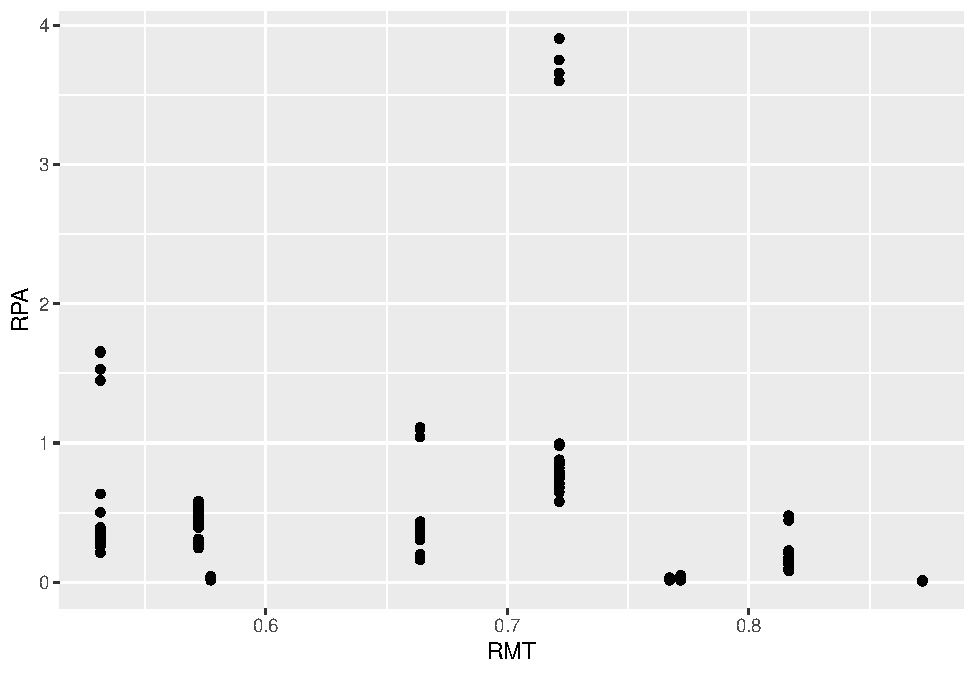
\includegraphics{FinalDeliverableArticle_files/figure-latex/unnamed-chunk-1-1.pdf}

\hypertarget{keywords}{%
\section{Keywords}\label{keywords}}

LaTex; R Markdown; Reproducable Research

\hypertarget{introduction}{%
\section{Introduction}\label{introduction}}

\hypertarget{background}{%
\paragraph{background}\label{background}}

In this template journal article, we will go through and explain how to
perform statistical analysis and data transformations. The Key features
we will discuss include, taking the mean of a dataset variable,
performing log transformations, inputing data into simple and complex
tables, how to format tables, introduction of math notation into the
article, plotting simple graphs along with more complex pinciple
component analysis graphs and heat map analysis as well as figure input
and layouts.

\hypertarget{mean-and-log-transformations}{%
\paragraph{Mean and Log
Transformations}\label{mean-and-log-transformations}}

Taking the mean of a data set is an important data transfermation that
is necessary in research practice before further statistical analysis
can be performed. The same can be said about log transformations. The
purpose in our research for performing a log transformation on our data
set is to create a set of values that are closer together. This is
necessary before you perform analysis such as PCA, as highly
differential variables will skewer PCA results and ofter prevent proper
clustering.

\begin{verbatim}
## $CF_1
## [1] 0.235109
## 
## $CF_2
## [1] 0.2507217
## 
## $CF_3
## [1] 0.3953087
## 
## $CF_4
## [1] 0.410819
## 
## $CF_5
## [1] 0.2038396
\end{verbatim}

\begin{verbatim}
##      CF_1      CF_2      CF_3      CF_4      CF_5 
## 0.2351090 0.2507217 0.3953087 0.4108190 0.2038396
\end{verbatim}

The log transformation of data can be done by first defining what we
want to transform, for example, the Relative Peak Areas (RPA) and
performing the function . This will perform the transformation, but in
order to visualize it you must thye the new transformed data's name
\emph{T\_log}

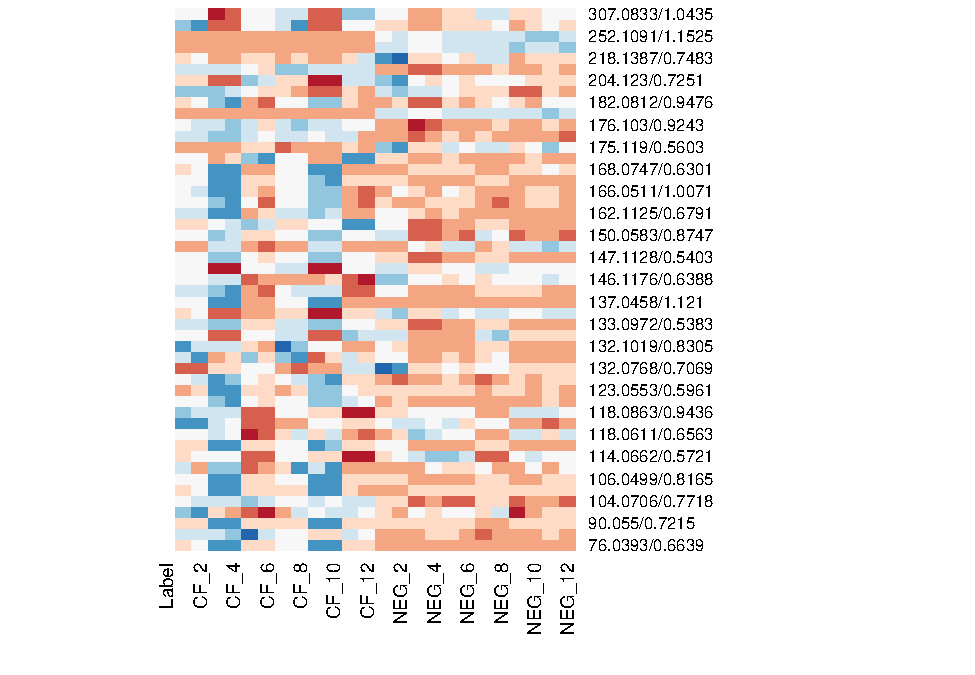
\includegraphics{FinalDeliverableArticle_files/figure-latex/unnamed-chunk-3-1.pdf}

\begin{Shaded}
\begin{Highlighting}[]
\KeywordTok{heatmap.2}\NormalTok{(Biomarker_Matrix, }\DataTypeTok{Rowv =} \OtherTok{NA}\NormalTok{, }\DataTypeTok{Colv =} \OtherTok{NA}\NormalTok{, }\DataTypeTok{scale =} \StringTok{"row"}\NormalTok{, }\DataTypeTok{density.info =} \StringTok{"none"}\NormalTok{, }\DataTypeTok{trace =} \StringTok{"none"}\NormalTok{, }\DataTypeTok{col =}  \KeywordTok{brewer.pal}\NormalTok{(}\DecValTok{11}\NormalTok{, }\StringTok{"RdBu"}\NormalTok{))}
\end{Highlighting}
\end{Shaded}

\begin{verbatim}
## Warning in heatmap.2(Biomarker_Matrix, Rowv = NA, Colv = NA, scale =
## "row", : Discrepancy: Rowv is FALSE, while dendrogram is `both'. Omitting
## row dendogram.
\end{verbatim}

\begin{verbatim}
## Warning in heatmap.2(Biomarker_Matrix, Rowv = NA, Colv = NA, scale =
## "row", : Discrepancy: Colv is FALSE, while dendrogram is `column'. Omitting
## column dendogram.
\end{verbatim}

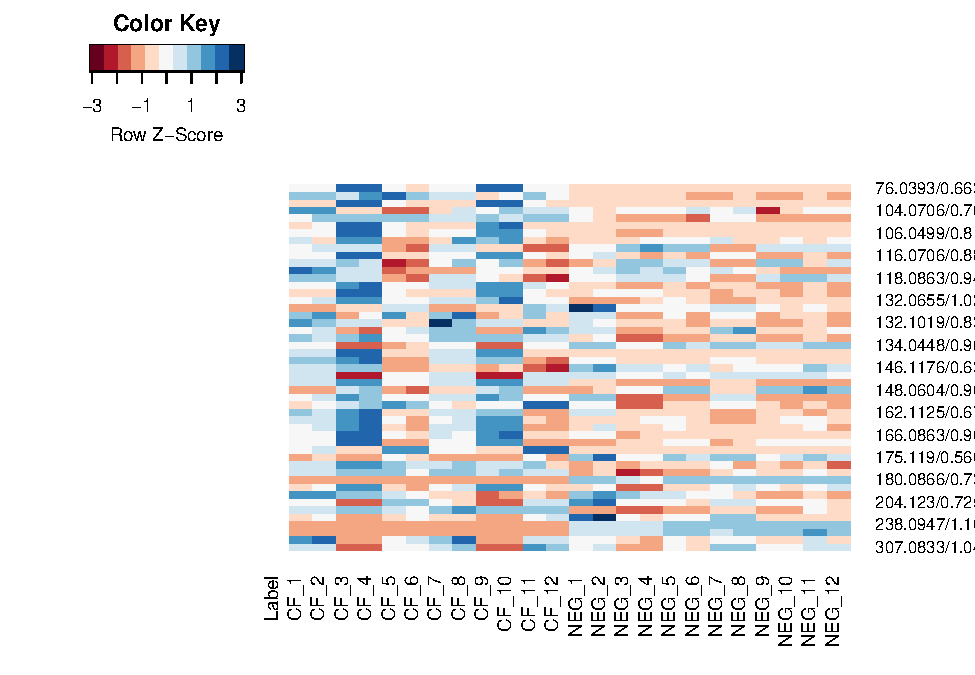
\includegraphics{FinalDeliverableArticle_files/figure-latex/unnamed-chunk-4-1.pdf}

\hypertarget{usage}{%
\paragraph{Usage}\label{usage}}

Once the package is properly installed, you can use the document class
\emph{elsarticle} to create a manuscript. Please make sure that your
manuscript follows the guidelines in the Guide for Authors of the
relevant journal. It is not necessary to typeset your manuscript in
exactly the same way as an article, unless you are submitting to a
camera-ready copy (CRC) journal.

\hypertarget{functionality}{%
\paragraph{Functionality}\label{functionality}}

The Elsevier article class is based on the standard article class and
supports almost all of the functionality of that class. In addition, it
features commands and options to format the

\begin{itemize}
\item
  document style
\item
  baselineskip
\item
  front matter
\item
  keywords and MSC codes
\item
  theorems, definitions and proofs
\item
  lables of enumerations
\item
  citation style and labeling.
\end{itemize}

\hypertarget{materials-and-methods}{%
\section{Materials and Methods}\label{materials-and-methods}}

\hypertarget{front-matter}{%
\section{Front matter}\label{front-matter}}

The author names and affiliations could be formatted in two ways:

\begin{enumerate}
\def\labelenumi{(\arabic{enumi})}
\item
  Group the authors per affiliation.
\item
  Use footnotes to indicate the affiliations.
\end{enumerate}

See the front matter of this document for examples. You are recommended
to conform your choice to the journal you are submitting to.

\hypertarget{bibliography-styles}{%
\section{Bibliography styles}\label{bibliography-styles}}

There are various bibliography styles available. You can select the
style of your choice in the preamble of this document. These styles are
Elsevier styles based on standard styles like Harvard and Vancouver.
Please use BibTeX~to generate your bibliography and include DOIs
whenever available.

Here are two sample references: Feynman and Vernon Jr. (1963; Dirac,
1953).

\hypertarget{references}{%
\section*{References}\label{references}}
\addcontentsline{toc}{section}{References}

\hypertarget{refs}{}
\leavevmode\hypertarget{ref-Dirac1953888}{}%
Dirac, P., 1953. The lorentz transformation and absolute time. Physica
19, 888--896.
doi:\href{https://doi.org/10.1016/S0031-8914(53)80099-6}{10.1016/S0031-8914(53)80099-6}

\leavevmode\hypertarget{ref-Feynman1963118}{}%
Feynman, R., Vernon Jr., F., 1963. The theory of a general quantum
system interacting with a linear dissipative system. Annals of Physics
24, 118--173.
doi:\href{https://doi.org/10.1016/0003-4916(63)90068-X}{10.1016/0003-4916(63)90068-X}


\end{document}


